% Chapter 5

\chapter{Galaxy Pairs, Mergers, and Morphologies} 
\label{Chapter:GalPairs}
\lhead{Chapter 5. \emph{Pairs, Mergers, and Morphologies}} 

$\Lambda$CDM cosmology predicts the hierarchical assembly of dark matter haloes.
Throughout the history of the Universe haloes have grown in mass and size via two pathways. 
Firstly haloes grow via smooth accretion gradually accreting dark matter from the surrounding environment. 
The secondary growth mechanism is via the accretion and gradual absorption of smaller haloes, known as subhaloes. 
After accretion subhaloes survive as substructure of the central/host halo gradually losing mass and sinking to the center of the potential well though dynamical friction. As discussed in previous Chapters these sub-haloes contain satellite galaxies that follow the halo structure causing galaxy galaxy mergers.

Frequent or massive mergers are thought to induce morphological changes in galaxies. 
Galaxies, after experiencing a massive merger, where the minor galaxy is at least a quarter of the mass of the central galaxy, are thought to lose their disk-like morphology and transform into elliptical galaxies \citep{Negroponte1983SimulationsGalaxies, DeLucia2006TheGalaxies}. 
For this reason it is important to understand the frequency and nature of mergers between galaxies to achieve a complete and coherent picture of galaxy formation and evolution. 
Unfortunately, galaxy mergers occur on gigayear timescales and therefore it is not possible to directly observe the rate or consequence of galaxy mergers. 
The traditional approach to estimate a measure of galaxy mergers is to count galaxy pairs at a given separation, and then assign a merging timescale to infer the rate of galaxy merging \citep{Conselice2003A3,Conselice2008TheField,Mundy2017A3.5,Duncan2019ObservationalFields}.
However, the approach of counting pairs is complicated by systematic differences when selecting galaxies, for example the evolution of the pair fraction appears to change if a selection is made by flux ratio or made by stellar mass ratio \citep{Man2016RESOLVING03}.

\section{The systematic effects of stellar mass estimation on galaxy pair fractions}

%What systemeatics can we expect to find in galaxy pairs (paper 3 plots 1,2,&3)

In this chapter we show how different SMHM relations generate distinct pair fractions and merger rates. 
Stellar mass functions with greater number densities of high-mass galaxies, naturally map larger galaxies into smaller haloes due to their higher relative abundances, resulting in steeper high-mass slopes for the SMHM relations.
In Figure \ref{fig:MassRatioCartoon} we show an illustrative cartoon of how different SMHM relations affect the galaxy mass ratios. 
For two identical mass halo pairs we see that a SMHM relation with a steeper slope causes a substantial difference in the stellar mass ratio that is mapped into the halo pairs. 

\begin{figure}[h]
	\centering
	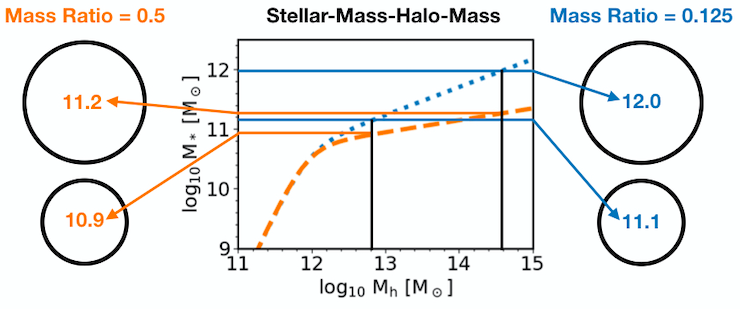
\includegraphics[width = \linewidth]{Figures/Chapter5/MassRatioCartoon.png}
	\caption{A cartoon showing the how the SMHM relation can impact the stellar mass ratio of galaxies mapped into identical halos. The steeper SMHM relation creates a smaller stellar mass ratio as the change in halo mass maps to a much larger stellar mass difference.}
	\label{fig:MassRatioCartoon}
\end{figure}

It follows that given two identical distributions of haloes seeded with galaxies via different SMHM relations the shallower one will seed more galaxy pairs\footnote{The pair fraction  defined here as the fraction of galaxies of a given mass that have a companion with a mass equal to or greater than a quarter of the primaries mass within 5-30 kpc.}.

In Figure \ref{fig:SMHM_PF_Cartoon} a cartoon is shown as an example of the expected difference in the pair fraction when changing the SMHM relation.
The left hand column shows the SMHM relations and the right column the pair fractions and their evolution with redshift. 
In the top row we compare a steep high-mass slope to a flatter slope, where the slope has been changed at redshift $z = 0.1$.
In the bottom row we compare an evolving and non-evolving high-mass slope.

\begin{figure}[h]
	\centering
	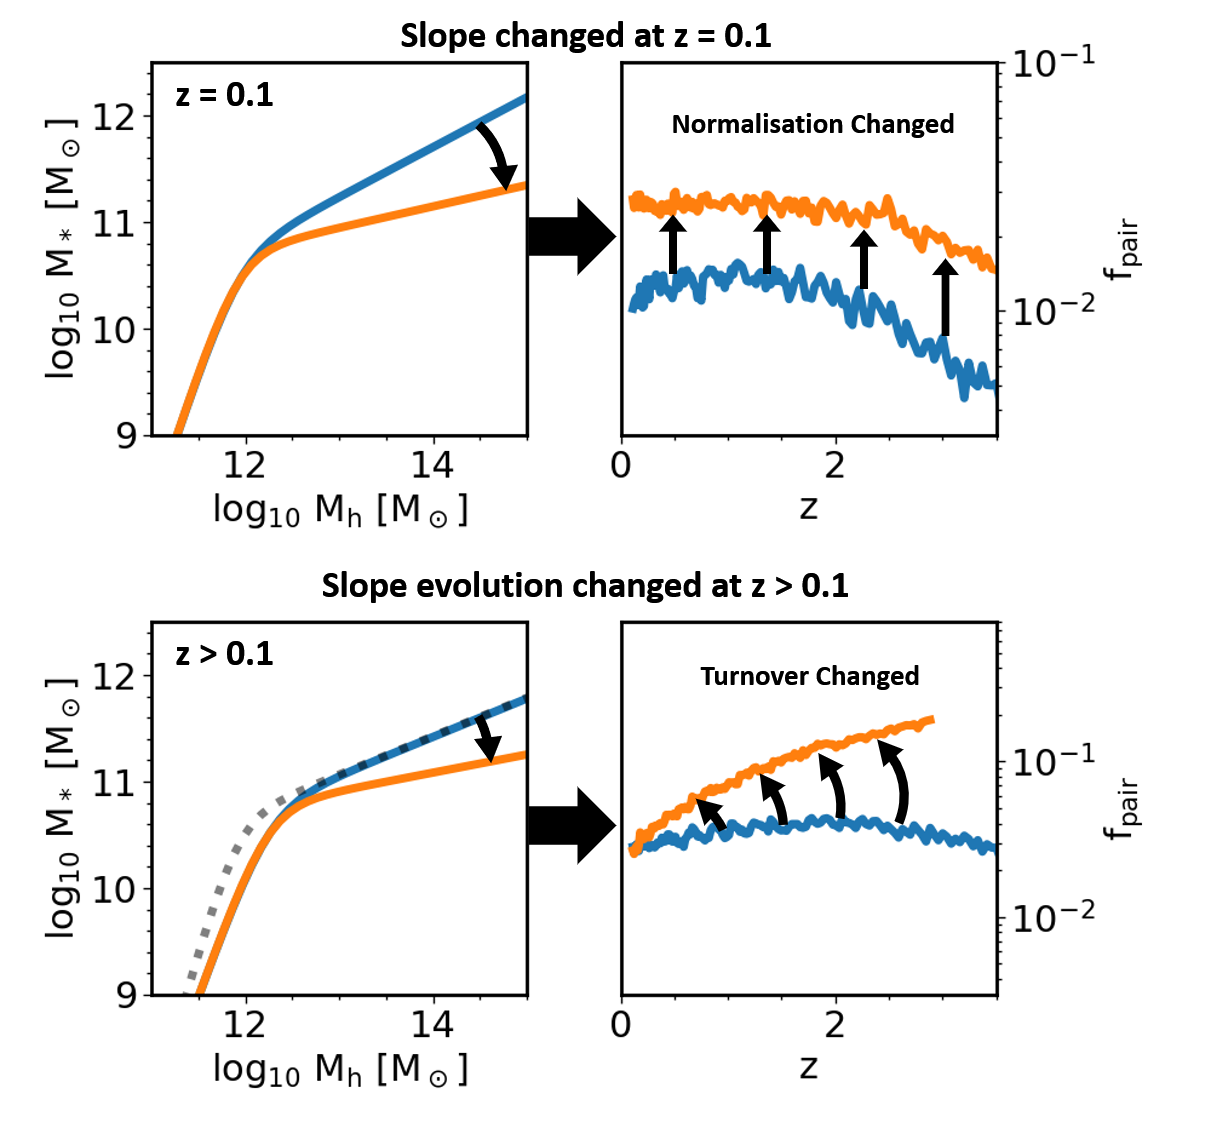
\includegraphics[width = \linewidth]{Figures/Chapter5/SMHM_PF_Cartoon.png}
	\caption{A cartoon showing the how the SMHM relation can impact the pair fraction. The top row shows how reducing the high mass slope of the SMHM relation increase the number of pairs at all redshifts. The bottom row shows the redshift $z=0$ relation as a grey dotted line, two relations at redshift where the relation is not evolved or evolved to be shallower are shown in blue and orange respectively. For this evolving SMHM relation the pair fractions are found to increase. In each case the reason for the increase can be explained by referencing Figure \ref{fig:MassRatioCartoon} where making the relation shallower seeds more massive pairs.}
	\label{fig:SMHM_PF_Cartoon}
\end{figure}

The steepening of the SMHM relation high-mass slope increases the number of pairs created and the normalisation of the pair fraction increases. 
In the bottom row we show the effects of having a slope that flattens at higher redshift. 
We show the redshift $z=0.1$ relation in grey and the relations with the unchanged and changed slopes in blue and orange respectively. 
The main effect of varying the evolution of the high-mass slope in the SMHM relation is to change the behaviour of pair fraction with redshift. 
A steeper slope tends to turn over the pair fraction and vice-versa.


The behaviours reported in Figure \ref{fig:SMHM_PF_Cartoon} are what one would expect given Figure \ref{fig:MassRatioCartoon}, where shallower slopes give higher fractions. 
Furthermore, from Figure \ref{fig:SMHM_PF_Cartoon} (and from Figure \ref{fig:PairFracSystematic}), it can be concluded that almost any pair fraction difference could be produced by appropriately altering the input SMHM relation. 
It is relevant to stress here that relatively minor changes in the stellar mass function can cause qualitative differences in the SMHM relation and, by extension, in the shape and normalization of pair fractions at any cosmic epoch.

The ability to systematically change the pair fraction due to stellar mass derivation calls to question the discrepancies found in pair fraction results \citep[e.g.][]{Man2016RESOLVING03}. 
If the pair fraction is systematically effected then where results do not use the same data processing then the difference could be due to non-trivial systematics. 
\steel as a flexible and lightweight model can illuminate the systematics by running with multiple input SMHM relations to test a range of different inputs and compare the results.

Calculation of the pair fraction in \steel requires an estimate of the distance between the central galaxy and the satellite galaxy, as we rely on our statistical accretion history, and do not have discrete halos, we assign each subhalo bin an average distance to the central galaxy. 
The subhaloes start at the viral radius of the central halo, the distance to the centre then reduces proportionally to the amount of dynamical time remaining \citep{Guo2011FromCosmology}.

To generate the systematic outputs a toy model where each of the main parameters (M, N, $\beta$, $\gamma$), and their evolutionary factors (M$_z$, N$_z$, $\beta_z$, $\gamma_z$), governing the SMHM relation are adjusted in turn to explore the affect on the galaxy pair fractions. Table \ref{tab:PairFracSysInput} details the change made to the SMHM relation for each parameter. 

\begin{table}
\centering
\caption{The adjustments to the SMHM relation used in Figure \ref{fig:PairFracSystematic}.}
\label{tab:PairFracSysInput}
\begin{tabular}{|c|cccc|} \hline
             & PyMorph   & $X_{0.1, alt}$  & $X_{z, +}$  & $X_{z, -}$  \\ \hline
$M$          & 11.92 & -0.25 & -     & -     \\ 
$M_{z}$      & 0.58   & -     & +0.1  & -0.1  \\ \hline
$N$          & 0.032 & +0.04 & -     & -     \\
$N_{z}$      & -0.014 & -     & +0.007 & -0.007 \\ \hline
$\beta$      & 1.64  & -0.3  & -     & -     \\
$\beta_{z}$  & -0.69  & -     & +0.3  & -0.3  \\ \hline
$\gamma$     & 0.53  & +0.06 & -     & -     \\
$\gamma_{z}$ & -0.03  & -     & +0.2  & -0.2  \\ \hline
\end{tabular}
\end{table}

Figure \ref{fig:PairFracSystematic} shows each of the SMHM relations in the outer four panels, the reference SMHM relation PyMorph is shown in blue at redshifts $z = 0.1$ (dotted line) and $z = 2$ (dashed line) in each panel, the modified redshift $z = 0.1$ relation is then shown in orange, and the increased and decreased (dashed red and green) evolution are shown at redshift $z = 2$. The inner four panels follow the same colour convention. 

\begin{landscape}
\begingroup
\begin{figure}[h]
	\centering
	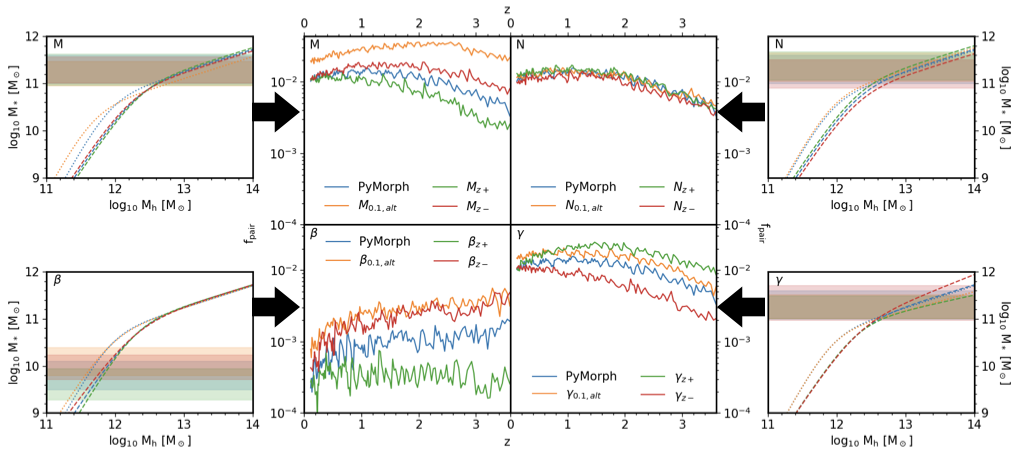
\includegraphics[width = \linewidth]{Figures/Chapter5/PairFractionSystematic.png}
	\caption{Each of the panel pairs (M, N, $\beta$, $\gamma$) shows the input SMHM relation in the outer plot and the modelled pair fraction evolution in the center plot. Each pair investigates adjustments to the given parameter of the SMHM relation (M, N, $\beta$, $\gamma$). Each pair shows the reference SMHM relation `G18' in blue, the relation adjusted at redshift $z = 0.1$ keeping the same SMHM relation evolution parameters in yellow. The red and green lines have the evolution parameter altered such that the evolution parameter is increased or decreased with respect to PyMorph respectively. In the outer (SMHM relation) plots dotted lines are $z = 0.1$ relations and dashed lines are $z = 2$ relations the PyMorph relation is shown at both epochs for comparison. Finally the shaded bands in the outer plots show the consistent number density selections used in the center plots.}
	\label{fig:PairFracSystematic}
\end{figure}
\endgroup
\end{landscape}

When changing M, the knee parameter, a large increase in the pair fraction is found from a lower knee: The shallower high mass slope is extended therefore more haloes are seeded in the mass range for pairs. 
We see the same effect at high redshift, the lower value of M at high redshift creates a higher pair fraction. 
The normalization parameter, N, creates little change in the pair fraction as expected because the mass ratios are largely unaffected. 
The low mass slope parameter, $\beta$, affects the seeding of smaller galaxies hence a lower mass range is used for the consistent number density cut. 
Due to the steepness of the low mass slope the fraction of pairs is lower in this mass cut.
Finally, when the high mass slope parameter, $\gamma$, is altered more pairs are found at high and low redshift when the slope is shallow. 
This is again attributed to more galaxies seeded within the mass ratio range.

\section{Galaxy Morphologies Resulting from Galaxy Mergers}
%What happens during a galaxy merger?

Galaxy mergers happen on timescales that dwarf human timescales when we observe galaxy mergers we see what equates to a static snapshot of the process. Much of our knowledge of galaxy mergers then comes from simulations of merging systems \cite[e..g.][]{Hopkins2006ASpheroids,Hopkins2009TheDemographics, Hopkins2010MergersRate,Hopkins2009HOWMERGERS,Hopkins2010MERGERSMATTER,OLeary2020EMERGE:zsim6,Fensch2017High-redshiftFormation,Stewart2008MergerSurvival,Stewart2009GALAXYDEPENDENCE}. Despite this wealth of simulation knowledge about the physics of galaxy mergers, the fulcrum of our understanding lies with the estimation of the rate and significance of mergers \cite{Hopkins2010MERGERSMATTER, Hopkins2010MergersRate}. Using the merger rates derived in Chapter \ref{Chapter:GalGrowth} we implement a post-processing method to ascertain the effects of traditional models when decoupled from merger trees and applied to true, statistical, populations in \steel.

%The fraction of elliptical galaxies stemming from galaxy major merger in steel
\subsection{Implementing discrete processes in a statistical model.}

One of the primary challenges in the development of \steel is trying to implement discrete processes in a statistical fashion. Mergers that happen between two galaxies are implemented stochastically using the following method.
\begin{itemize}
    \item At each time-step for each central halo mass track the mass bins of previously accreted subhalo/satellite galaxy mass functions that have reached the end of their dynamical time are summed to produce the merging satellite stellar mass function. 
    \item Each central halo mass track is assigned a central stellar mass at each epoch $M_{*,cent}(M_{h}, z)$ (Figure \ref{fig:Cent_Mass_PP}). By integrating the merging satellite stellar mass function in the range [$M_{*,cent}(M_{h}, z) \cdot \mu$, $M_{*,cent}(M_{h}, z)$] the probability that a given central has undergone a major merger at each epoch is retrieved, where $\mu$ is the major merger mass ratio. 
    \item In Figure \ref{fig:Gal_Morph_toon} an illustration of the way galaxy morphologies are updated is given. 
    \begin{itemize}
        \item In the leftmost panel all galaxies are spirals or a disk like morphology (blue bar), the probability of a galaxy having a major merger is shown as a black line.
        \item Following the arrow to the middle panel the fraction of galaxies that had a major merger are assigned as ellipticals. The mass track at this epoch now has this spiral to elliptical ratio.
        \item At this next time step the fraction of galaxies undergoing a major merger is calculated, however, this is split between galaxies that have previously had a major merger and those that have not. 
        \item Following the arrow from the middle to the right hand panel we see only the galaxies that were in the spiral group contribute to the increased elliptical fraction.
        \item Using this process at each time-step eventually all galaxies can become elliptical but the rate at which this happens slows.
    \end{itemize}
    \item Using the process as described we can apply discrete processes to mass tracks that describe a diverse population.
\end{itemize}

\begin{figure}[h]
	\centering
	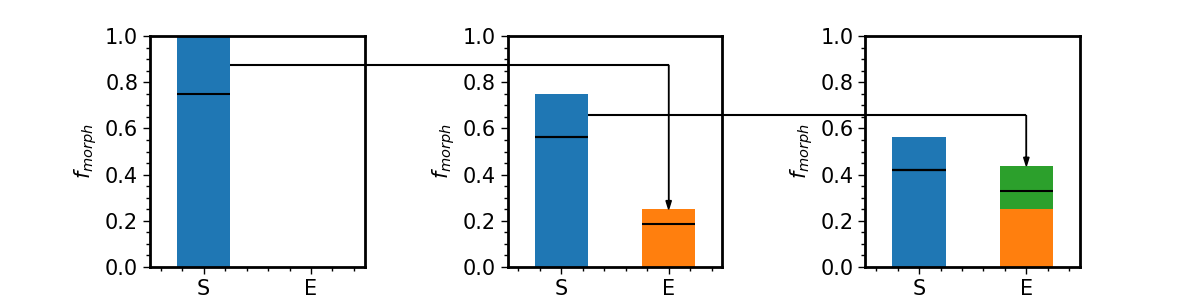
\includegraphics[width = \linewidth]{Figures/Chapter5/Morphology_Evolution.png}
	\caption{A cartoon of the way we assign morphologies statistically in $\steel$. Each step has the same fraction of major mergers but the number of ellipticals created reduces as some major mergers occur on the elliptical fraction. The fraction of galaxies in each population experiencing a major merger is displayed as a horizontal black line.}
	\label{fig:Gal_Morph_toon}
\end{figure}

Applying the above process to galaxies in \steel from redshift $z = 3$ we obtain the morphological fraction of galaxies at different masses using a major mass ratio of $\mu = 0.25$, at redshifts $z = 0.1, 0.65, 1.75$. Figure \ref{fig:Gal_Morph} shows the probability/fraction of central galaxies that have elliptical morphologies, while the black triangles show the T-Type-selected elliptical fraction from the SDSS catalogue. We find that applying this simple recipe to the merging number densities from \textsc{steel} creates a good match to the elliptical fraction in the local universe.

\begin{figure}[h]
	\centering
	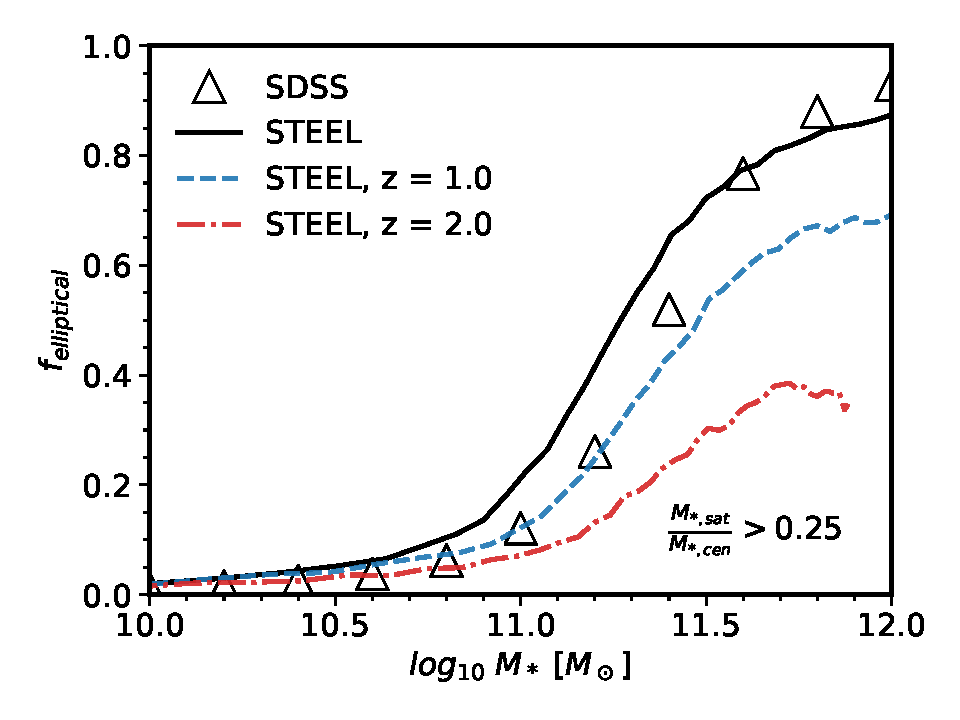
\includegraphics[width = \linewidth]{Figures/Chapter5/GalaxyMorphologies.pdf}
	\caption{We show at three redshift steps the predicted fraction of ellipticals as a function of stellar mass. The lines are the predictions from \textsc{steel} and the triangles are the T-Type selected elliptical fraction from SDSS at redshift $z = 0.1$.}
	\label{fig:Gal_Morph}
\end{figure}


\section{Lenticular Galaxy Formation}
%What is a lenticular and why are they considered independently to the rest of the galaxy population?
%What have been the proposed models of Lenticular formation?
%Building a least assumption model of lenticular formation (supervised project)